% TU Delft beamer template
% Author: Erwin Walraven (initial version was created by Maarten Abbink)
% Delft Universiy of Technology

\documentclass{beamer}
\usepackage[english]{babel}
\usepackage{calc}
\usepackage[absolute,overlay]{textpos}
\usepackage{graphicx}
\graphicspath{{../figures/}}
\usepackage{subfig}
\usepackage{amsmath}
\usepackage{amsfonts}
\usepackage{amsthm}
\usepackage{mathtools}
\usepackage{comment}
\usepackage{MnSymbol,wasysym}
\usepackage[noend]{algpseudocode}
\usepackage{algorithm}

\setbeamertemplate{navigation symbols}{} % remove navigation symbols
\mode<presentation>{\usetheme{tud}}

\newcommand{\A}{\mathcal{A}}
\newcommand{\C}{\mathcal{C}}
\renewcommand{\P}{\mathcal{P}}
\newcommand{\F}{\mathcal{F}}
\newcommand{\E}{\mathcal{E}}

\algnewcommand\algorithmicupon{\textbf{Upon}}
\algnewcommand\Upon{\item[\algorithmicupon]}

\algnewcommand\algorithmicsend{\textbf{Send}}
\algnewcommand\Send{\item[\algorithmicsend]}

% \setbeameroption{show notes}

\title{Blockchain Consensus Protocol with\\Horizontal Scalability}
% \subtitle{Optional Subtitle}

\author{K.~Cong}
% - Give the names in the same order as the appear in the paper.
% - Use the \inst{?} command only if the authors have different
%   affiliation.

\institute[Delft University of Technology] % (optional, but mostly needed)
{
  Faculty of Electrical Engineering, Mathematics and Computer Science\\
  Delft University of Technology}
% - Use the \inst command only if there are several affiliations.
% - Keep it simple, no one is interested in your street address.

% \date{Conference Name, 2013}
\date{\today}

\AtBeginSubsection[] % Do nothing for \subsection*
{
  % do nothing
}

\AtBeginSection[] % Do nothing for \section*
{
  \begin{frame}<beamer>
  \frametitle{Outline}
  \tableofcontents[currentsection]
  \end{frame}
}


% Let's get started
\begin{document}

\begin{frame}
  \titlepage

\end{frame}

\begin{frame}{Outline}
  \tableofcontents
  % You might wish to add the option [pausesections]
\end{frame}

% Section and subsections will appear in the presentation overview
% and table of contents.
\section{Introduction}
\begin{frame}{Motivation}
  \begin{itemize}
    \item Blockchain systems offer an alternative to central authorities for the first time
    \item Market cap (40 billion for Bitcoin) and trade volume figures indicate they are here to stay
    \item Early blockchain systems are not scalable (7 TX/s for Bitcoin)
    \item Parameter tuning leads to centralisation
  \end{itemize}
\end{frame}

\begin{frame}{Research question}
  \begin{block}{}
    How do we design a \emph{blockchain consensus protocol} that is \emph{fault tolerant},
    \emph{scalable} and can reach \emph{global consensus?}
  \end{block}
    \note{
      \begin{itemize}
      \item Blockchain consensus protocol---independent of the application, like PoW (not PoS)
      \item Byzantine fault tolerance---if some number of nodes are malicious then the system should continue to function
      \item Horizontal scalability---if every node make transactions at the same rate, then the global throughput should increase
      \item Global consensus---all node should agree on a global state, useful for some applications, e.g. digital cash
      \end{itemize}
    }
\end{frame}

\begin{frame}{Inspiration}
  \begin{itemize}
    \item A restaurant owner does not report all of its transactions with an central authority
    \item Occasionally a customer may leave without paying and this event is reported to a central authority
    \item Our blockchain system achieves scalability using a similar idea
  \end{itemize}
\end{frame}

\section{System architecture}
\subsection{System model}
\begin{frame}{\subsecname}
  \begin{itemize}
    \item Population size is $N$
    \item $n$ nodes are facilitators, $t$ nodes are malicious (Byzantine)
    \item $n \ge 3t + 1$
    \item $N \ge n + t$
    \item Purely asynchronous channels with eventual delivery
    \item Public key infrastructure
    \item Random oracle model
    \item Computational security
  \end{itemize}
  \note{At this point, explain facilitators are nodes that have some extra task to do, temporarily.}
\end{frame}

\subsection{Architecture overview}
\begin{frame}{\subsecname}
  \begin{figure}[h]
  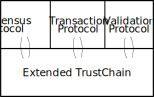
\includegraphics[width=0.7\textwidth]{architecture}
  \centering
  \end{figure}
  \note{
    \begin{itemize}
    \item The primary data structure is the Extended TrustChain, extension of our prior work
    \item The three protocols the tasks as their name suggests
    \item They are independent and run concurrently
    \item The only synchronisation happens via the Extended TrustChain
    \item But in no part of those protocol do we lock the Extended TrustChain
    \end{itemize}
  }
\end{frame}

\subsection{Extended TrustChain}
\begin{frame}{\subsecname}
  \begin{itemize}
    \item Everyone has their own chain and genesis block
    \item Two types of blocks
      \begin{enumerate}
      \item Transaction (TX) block
      \item Checkpoint (CP) block
      \end{enumerate}
    \item A transaction involves two parties and results in two TX blocks (a pair)
    \item A CP block captures the chain state
    \item TX and CP blocks are chained together using hash pointers
  \end{itemize}
\end{frame}

\begin{frame}{\subsecname}
  \begin{figure}[h]
  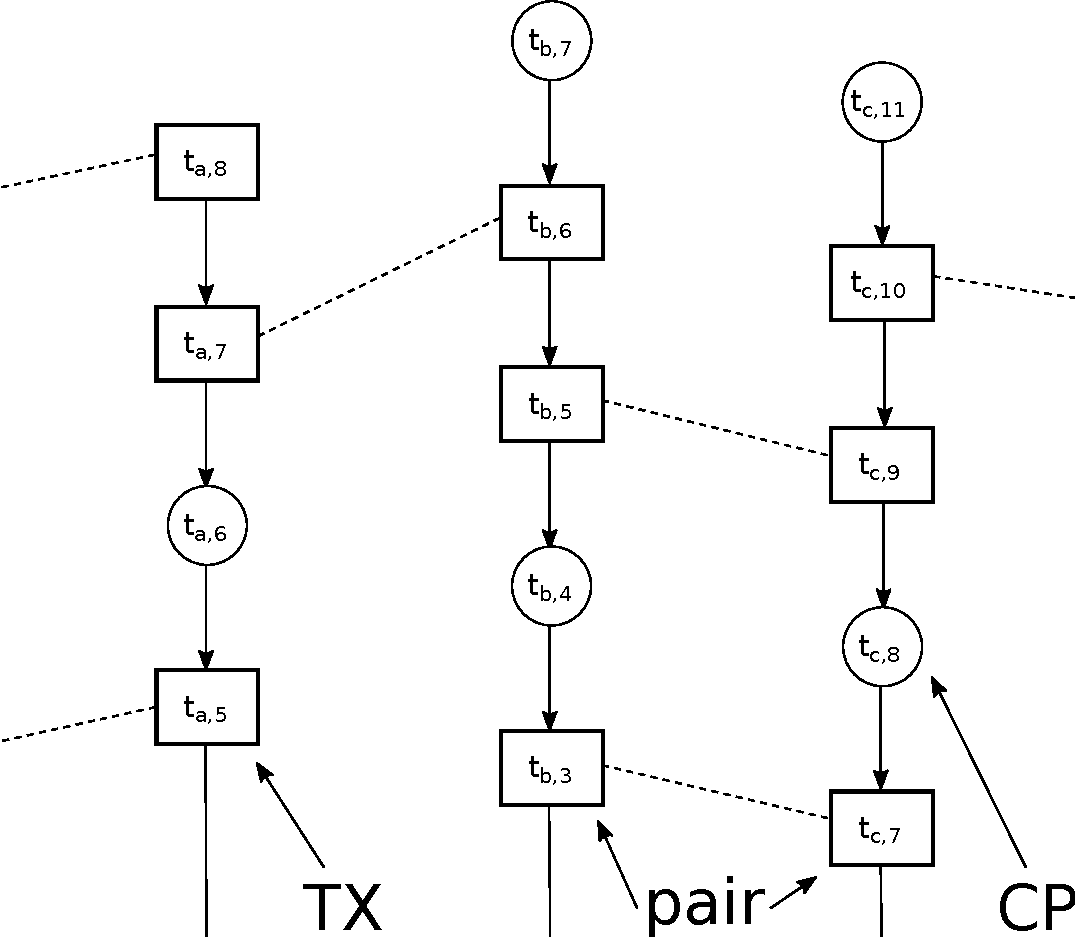
\includegraphics[width=0.67\textwidth]{trustchain-good-cp}
  \centering
  \caption{TX block is a six-tuple: $t_{u, i} = \langle \textsf{H}(b_{u, i - 1}), i, txid, pk_v, m, sig_u \rangle$.
    CP block is a five-tuple: $c_{u, i} = \langle \textsf{H}(b_{u, i-1}), i, \textsf{H}(\C_r), r, sig_u \rangle$.}
  \end{figure}
  \note{
    \begin{itemize}
      \item In this example there are three nodes
      \item Squares are TX blocks and circles are CP blocks
      \item Explain the block content in caption
      \item The dotted line represent pairs of TX blocks
      \item Geared with the understanding of our data structure, we are ready to talk about the consensus protocol
    \end{itemize}
  }
\end{frame}

\begin{frame}{\subsecname:~fragment definition}
\begin{itemize}
\item A fragment $F_{u, i}$ is defined on a TX block $t_{u, i}$
\item It is a section of the chain beginning and ending with CP blocks that contains the TX
\end{itemize}
\end{frame}

\subsection{Consensus protocol}
\begin{frame}{\subsecname:~overview}
  \begin{enumerate}
    \item Runs in rounds
    \item In round $r$, $n$ out of $N$ act as facilitators
    \item The facilitators collect CP blocks from all nodes
    \item Facilitators run a Byzantine consensus algorithm to agree on a set of CP blocks
    \item Disseminate the consensus result $\C_r$, i.e. the CP blocks
    \item From $\C_r$, new facilitators are computed
    \item Repeat
  \end{enumerate}
\end{frame}

\begin{frame}{\subsecname:~properties}
\label{def:consensus}
$\forall r \in \mathbb{N}$, the following properties must hold.
\begin{itemize}
    \item \emph{Agreement}:
        If one correct node outputs a set of facilitators $\F_r$,
        then every node outputs $\F_r$
    \item \emph{Validity}:
        If any correct node outputs $\F_r$, then 
            \begin{enumerate}
                \item $|\C_r| \ge N - t$ must hold for the $\C_r$ which was used to create $\F_r$,
                \item $\F_r$ must contain at least $n - t$ honest nodes and
                \item $|\F_r| = n$.
            \end{enumerate}
    \item \emph{Fairness}:
        Every node with a CP block in $\C_r$ should have an equal probability of becoming a member of $\F_r$.
    \item \emph{Termination}:
        Every correct node eventually outputs some $\F_r$.
\end{itemize}
\end{frame}

\begin{frame}{\subsecname}
  \begin{figure}[h]
  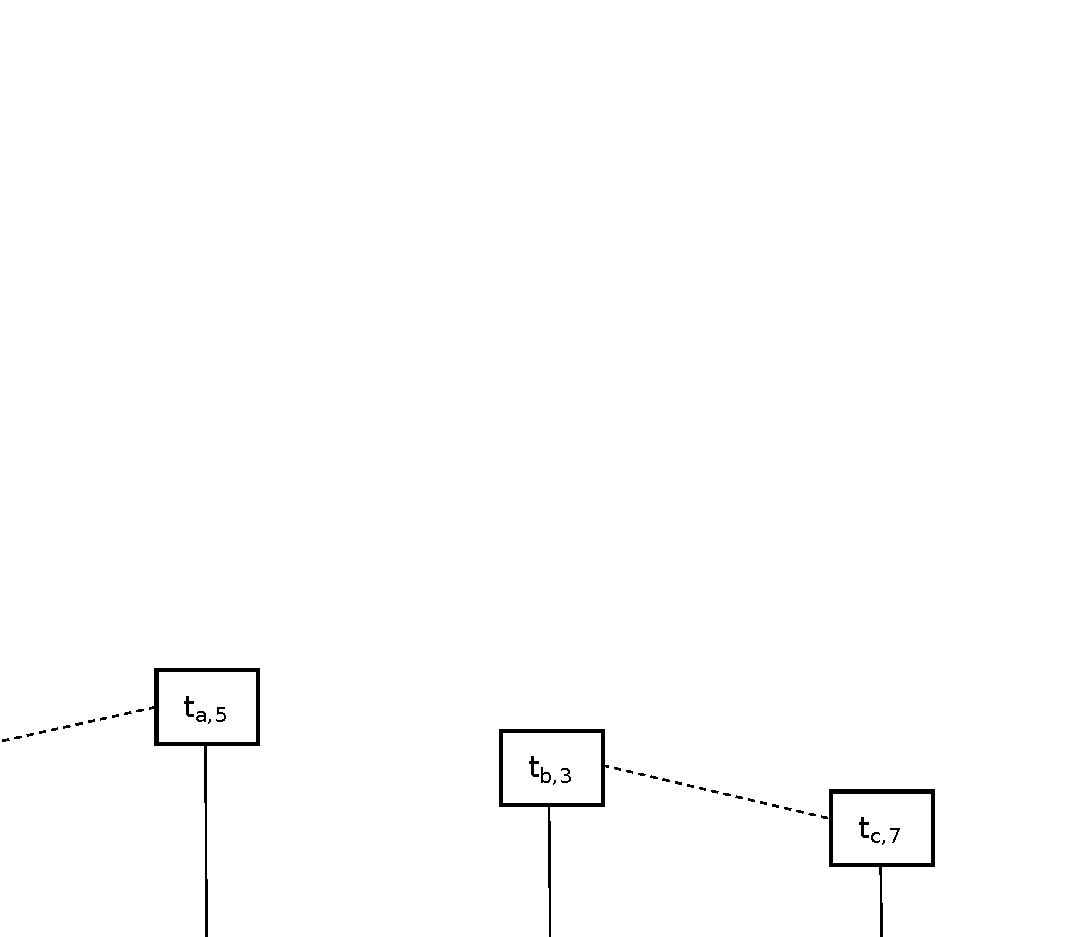
\includegraphics[width=0.67\textwidth]{trustchain-1}
  \centering
  \caption{Suppose we are in a state where $\C_{r - 1}$ has just been agreed by some facilitators but not yet propagated.}
  \end{figure}
\end{frame}

\begin{frame}{\subsecname}
  \begin{figure}[h]
  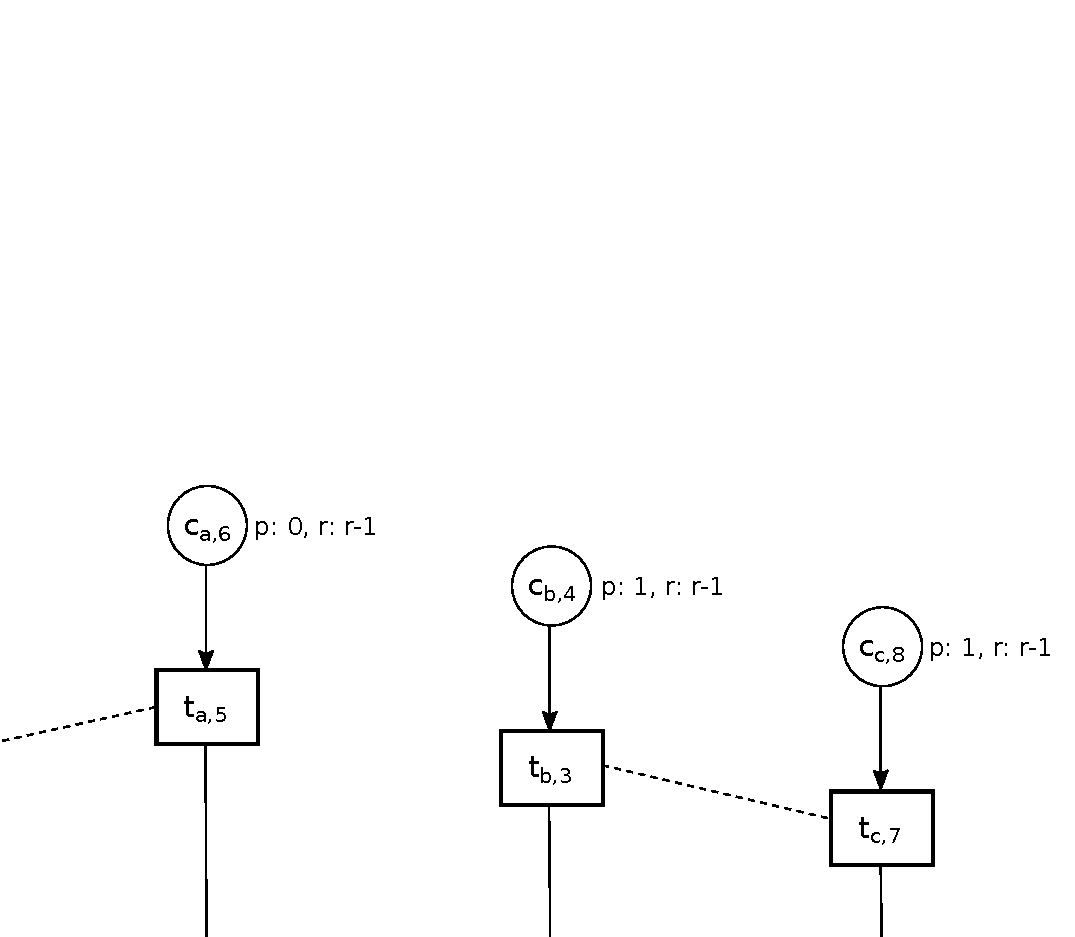
\includegraphics[width=0.67\textwidth]{trustchain-2}
  \centering
  \caption{Nodes receive consensus result $\C_{r - 1}$,
    first $n$ nodes ordered by $\textsf{H}(\C_{r-1} || pk)$ become $\F_{r-1}$,
    send the new CP blocks to $\F_{r-1}$.}
  \end{figure}
\end{frame}

\begin{frame}{\subsecname}
  \begin{figure}[h]
  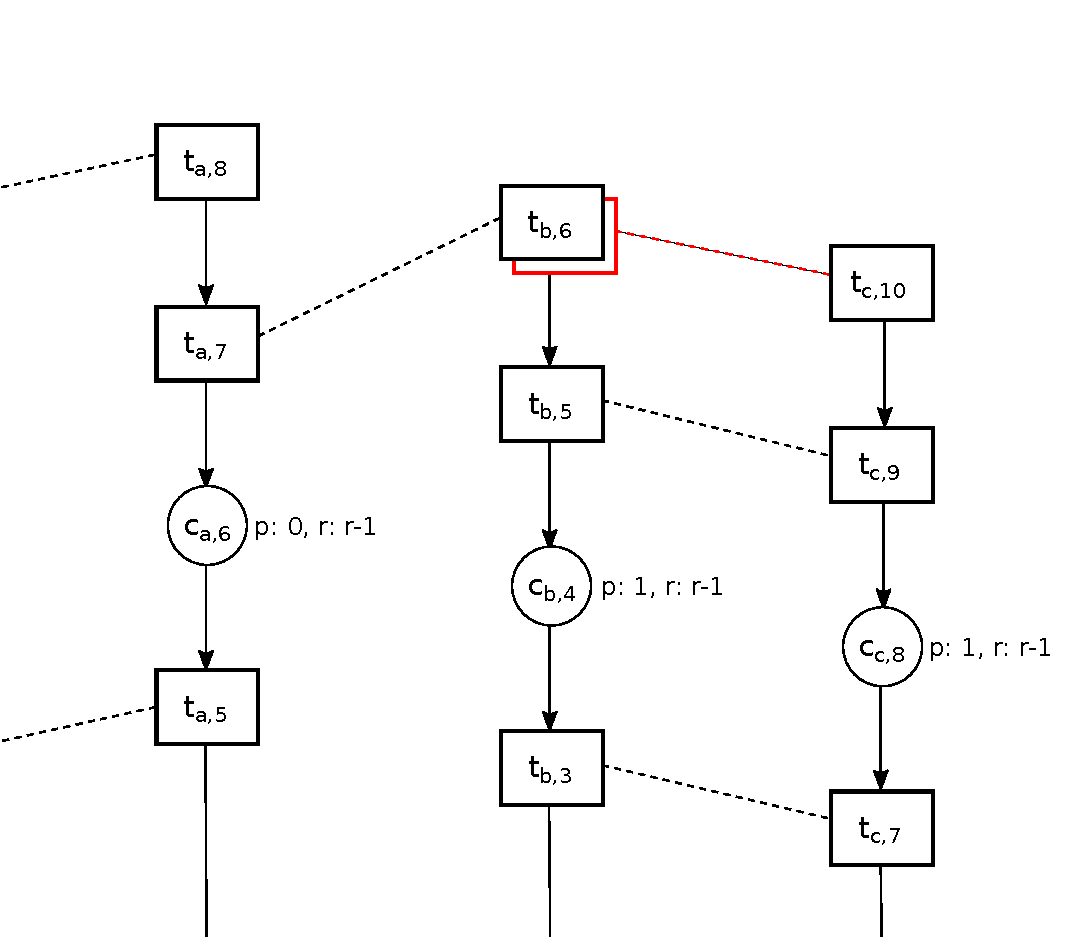
\includegraphics[width=0.67\textwidth]{trustchain-3}
  \centering
  \caption{Transactions carry on as usual in round $r$,
  while facilitators are trying to reach consensus on the new CP blocks concurrently.}
  \end{figure}
\end{frame}

\begin{frame}{\subsecname}
  \begin{figure}[h]
  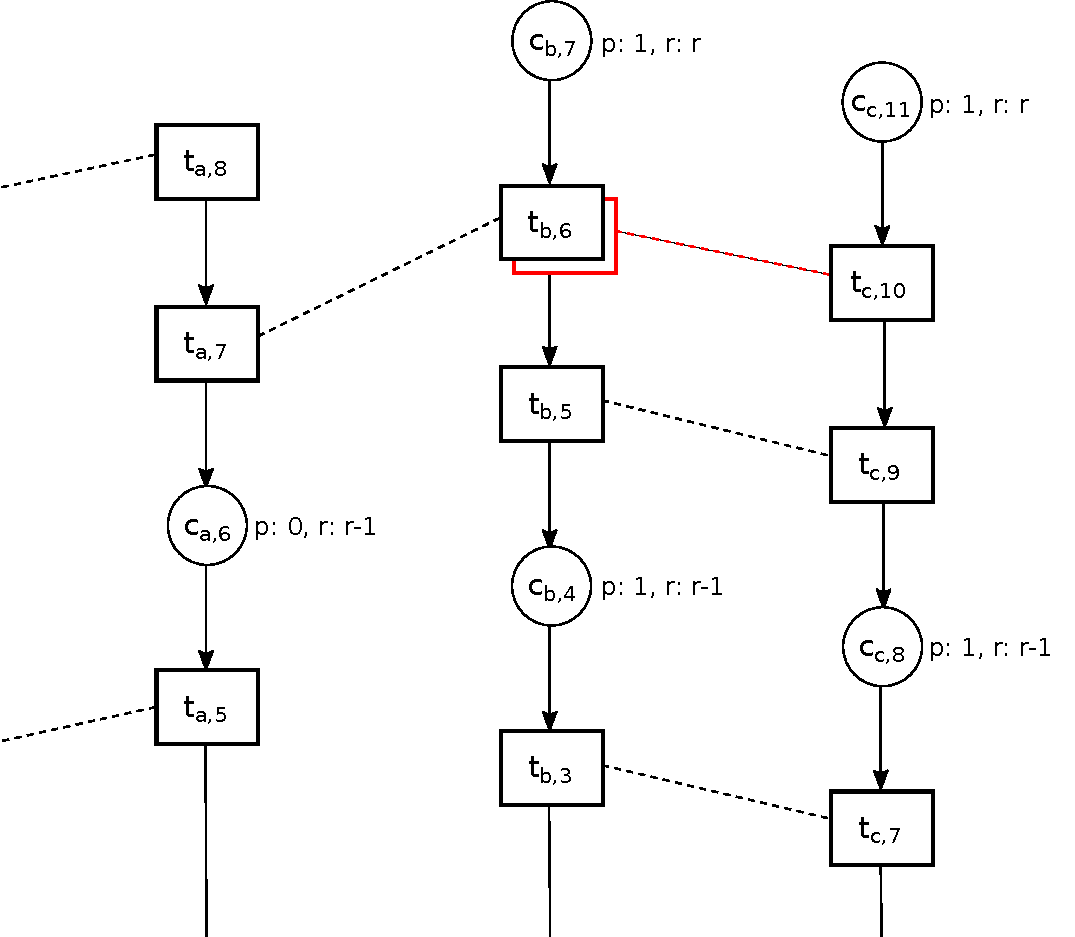
\includegraphics[width=0.67\textwidth]{trustchain-4}
  \centering
  \caption{$\F_{r-1}$ agree and disseminate $\C_r$,
  CP blocks at round $r-1$ ($c_{a, 6}, c_{b, 4}, c_{c,8}$) should be in $\C_r$.}
  \end{figure}
\end{frame}

\subsection{Transaction protocol}
\begin{frame}{\subsecname}
\begin{itemize}
\item Request (\texttt{tx\_req}) and response (\texttt{tx\_resp}) protocol
\item Two TX blocks containing the same $txid$ are generated
\item Non-blocking
\end{itemize}
\end{frame}

\begin{frame}{\subsecname}
Create $t_{u, h}$ and send $\langle \texttt{tx\_req}, t_{u, h} \rangle$ to start a transaction.
\vspace{5 mm}
\begin{algorithmic}
    \Upon $\langle \texttt{tx\_req}, t_{v, j} \rangle$ from $v$
    \State $\langle \_, \_, txid, pk_v, m, \_ \rangle \gets t_{v, j}$ \Comment unpack $t_{v, j}$
    \State $\textsf{new\_tx}(pk_u, m, txid)$ \Comment create and store $t_{u, i}$
    \State store $t_{v, j}$ as the pair of $t_{u, h}$
    \State send $\langle \texttt{tx\_resp}, t_{u, h} \rangle$ to $v$

    \Upon $\langle \texttt{tx\_resp}, t_{v, j} \rangle$ from $v$  
    \State $\langle \_, \_, txid, pk_v, m, \_ \rangle \gets t_{v, j}$ \Comment unpack $t_{v, j}$
    \State store $t_{v, j}$ as the pair of the TX with identifier $txid$
\end{algorithmic}
\end{frame}

\subsection{Validation protocol}
\begin{frame}{\subsecname:~overview}
\begin{itemize}
\item Request (\texttt{vd\_req}) and response (\texttt{vd\_resp}) protocol
\item Transactions are in three states---\emph{valid}, \emph{invalid} and \emph{unknown}---defined by $\textsf{get\_validity}(\cdot)$
\item The goal is to identify which state a given transaction is in satisfying the validation protocol properties
\end{itemize}
\end{frame}

\begin{frame}{Validity definition}
\textbf{Function} $\textsf{get\_validity}(t_{u, i}, F)$ validates the transaction $t_{u, i}$
\vspace{5 mm}
\begin{algorithmic}
    \State Check that $v$ sent the correct $F$,
    otherwise return \emph{unknown}.

    \State
    \State $\langle \_, \_, txid, pk_v, m, \_ \rangle \gets t_{u, i}$
    \If{number of blocks of $txid$ in $F \ne 1$}
        \State \Return \emph{invalid}
    \EndIf
    \State \Comment TX exists 

    \State $\langle \_, \_, txid', pk'_u, m', \_ \rangle \gets t_{v, j}$
    \If{$m \ne m' \vee pk_u \ne pk'_u$}
        \State \Return \emph{invalid}
    \EndIf
    \State \Comment no tampering
    \State \Return \emph{valid}
\end{algorithmic}
\end{frame}

\begin{frame}{\subsecname:~properties}
\begin{itemize}
    \item \emph{Agreement}:
        If any correct node decides on the validity of a transaction (except when it is \emph{unknown}),
        then all other correct nodes are able to reach the same conclusion or \emph{unknown}.
    \item \emph{Correctness}:
        The validation protocol outputs the correct result
        according to the aforementioned validity definition.
    \item \emph{Liveness}:
        Any valid (invalid) transaction is marked as validated (invalid) eventually.
\end{itemize}
\note{Liveness is not possible in our case because malicious nodes can simply go offline or refuse to respond,
but the other two properties are possible.}
\end{frame}

\begin{frame}{\subsecname}
Send $\langle \texttt{vd\_req}, txid \rangle$ to $v$ to begin.
\vspace{5 mm}
\begin{algorithmic}
    \Upon $\langle \texttt{vd\_req}, txid \rangle$ from $v$
        \State $t_{u, i} \gets \text{the transaction identified by } txid$
        \State $F_{u, i} \gets \textsf{agreed\_fragment}(t_{u, i})$
        \State send $\langle \texttt{vd\_resp}, txid, F_{u, i} \rangle$ to $v$

    \Upon $\langle \texttt{vd\_resp}, txid, F_{v, j} \rangle$ from $v$
        \State $t_{u, i} \gets \text{the transaction identified by } txid$
        \State set the validity of $t_{u, i}$ to $\textsf{get\_validity}(t_{u, i}, F_{v, j})$
\end{algorithmic}
\end{frame}

\section{Analysis of correctness and performance}

\subsection{Correctness of the consensus protocol}
\begin{frame}{\subsecname}
\begin{theorem}
For all rounds,
the consensus protocol satisfies agreement, validity, fairness and termination properties.
\end{theorem}
\begin{proof}(sketch)
Because consensus result are eventually delivered and the properties of Byzantine consensus,
we get agreement, validity and termination.
Fairness is from the fact that we model $\textsf{H}(\cdot)$ as a random oracle (RO) and the input to the RO is different for every node,
thus the list of nodes ordered by $\textsf{H}(\C_r || pk )$ is a random permutation of those nodes.
\end{proof}
\end{frame}

\subsection{Correctness of the validation protocol}
\begin{frame}{\subsecname}
\begin{theorem}
  The validation protocol satisfies agreement and correctness properties.
\end{theorem}
\begin{proof}(sketch)
Proof by contradiction.
For this attack to work, the adversary must be able to create two different fragments but with the same checkpoint enclosure.
We model $\textsf{H}(\cdot)$ as a RO, so the adversary need to query the RO a exponential\footnote{In terms of the security parameter.} number of times.
But the adversary can only query the RO a polynomial number of times.
Hence we have agreement.
Correctness follows directly the use of the $\textsf{get\_validity}(\cdot)$ function.
\end{proof}
\end{frame}

\subsection{Linear global throughput argument}
\begin{frame}{\subsecname}
\begin{itemize}
  \item Throughput has a notion of time but our model is asynchronous
  \item Additional assumptions needed to make the argument---every unit of communication takes a non-negligible amount of time to process
  \item Bandwidth relation---$NC \ge r_{\text{tx}} l$, where $l$ is $O(N)$
  \item If $r_\text{tx}$ satisfies the inequality, then LHS and RHS grows at the same rate,
  thus we have linear global throughput
\end{itemize}
\end{frame}

\section{Experimental results}
\begin{frame}{Implementation and experiment setup}
  \begin{itemize}
    \item Prototype implementation on Github\footnote{\url{https://github.com/kc1212/consensus-thesis-code}}
    \item SHA256 for hash functions and Ed25519 for digital signature
    \item Experiment on the DAS-5\footnote{\url{http://www.cs.vu.nl/das5/}}
      \begin{itemize}
        \item Up to 30 machines
        \item Each running 40 nodes
      \end{itemize}
  \end{itemize}
\end{frame}

\begin{frame}{Throughput vs population size (random neighbour)}
  \begin{figure}[h]
  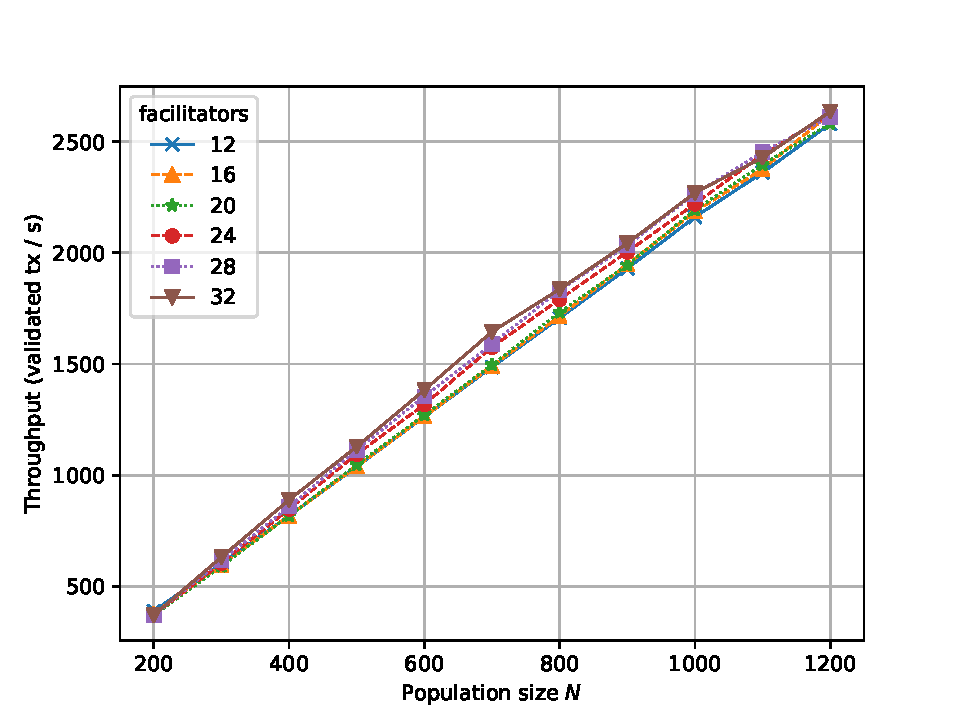
\includegraphics[width=0.9\textwidth]{neighbour-random/throughput-vs-population}
  \centering
  \end{figure}
\end{frame}

\begin{frame}{Throughput vs population size (fixed neighbour)}
  \begin{figure}[h]
  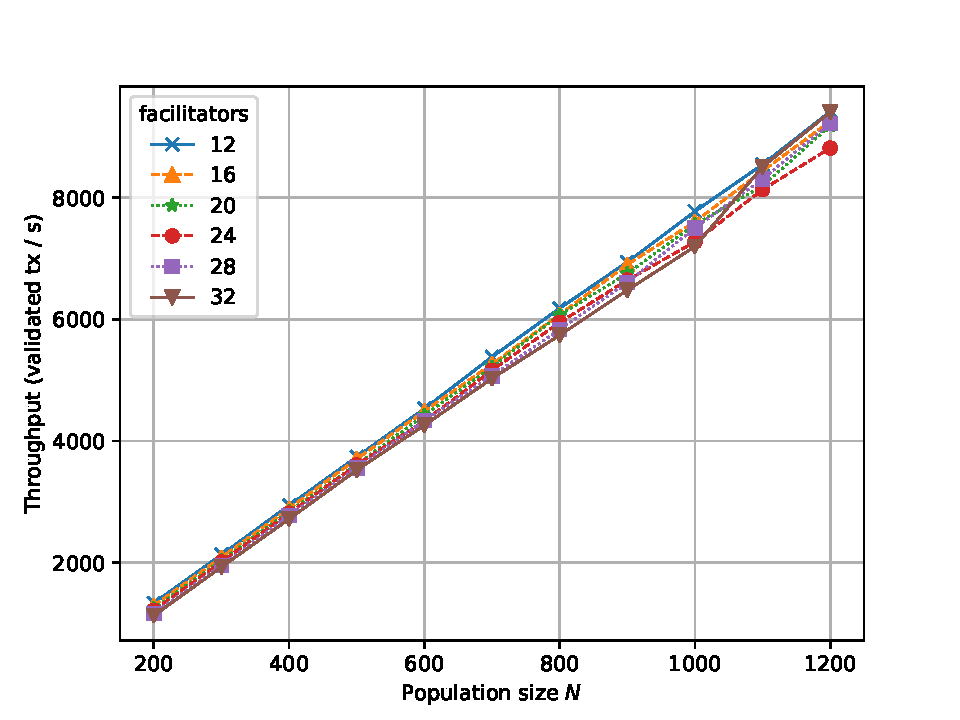
\includegraphics[width=0.9\textwidth]{neighbour-fixed/throughput-vs-population}
  \centering
  \end{figure}
\note{No need to request for fragment every time a TX needs to be validated. Upon receiving a fragment, validate as many TX as possible.}
\end{frame}

\section{Conclusion}
\begin{frame}{\secname}
  \begin{block}{Research question}
    How do we design a \emph{blockchain consensus protocol} that is \emph{fault tolerant},
    \emph{scalable} and can reach \emph{global consensus?}
  \end{block}
Our system achieve the following
\begin{itemize}
  \item Fault tolerant up to $t$ nodes
  \item Horizontal scalability
  \item Global consensus on CP blocks
\end{itemize}
\end{frame}

\begin{frame}{Future work}
\begin{itemize}
\item Improve fault tolerance
\item Improve fork detection
\item Analyse the system in the permissionless environment
\item Concrete application
\end{itemize}
\end{frame}

\end{document}

